\documentclass[a4paper,11pt]{kth-mag}
\usepackage[T1]{fontenc}
\usepackage{textcomp}
\usepackage{lmodern}
\usepackage[latin1]{inputenc}
\usepackage[swedish,english]{babel}
\usepackage{modifications}

\usepackage{graphicx}
\usepackage{amsmath}
\usepackage{bm}

% Put title here
\title{Weakly Supervised Object Detection: (Working title)}

\subtitle{Duis autem vel eum iruire dolor in hendrerit in
          vulputate velit esse molestie consequat, vel illum
          dolore eu feugiat null}
\foreigntitle{Lorem ipsum dolor sit amet, sed diam nonummy nibh eui
              mod tincidunt ut laoreet dol}
              
\author{Muhammad Iqbal Tawakal}

\date{2015}
\blurb{Master's Thesis at NADA\\Supervisor: Tjoho\\Examiner: Tjohej}
\trita{TRITA xxx yyyy-nn}

\begin{document}
\frontmatter
\pagestyle{empty}
\removepagenumbers
\maketitle
\selectlanguage{english}

\begin{abstract}
  This is a skeleton for KTH theses. More documentation
  regardings the KTH thesis class file can be found in
  the package documentation.
  
  Weakly supervised object detection is...
\end{abstract}

\clearpage
\begin{foreignabstract}{swedish}
  Denna fil ger ett avhandlingsskelett.
  Mer information om \LaTeX-mallen finns i
  dokumentationen till paketet.

\end{foreignabstract}
\clearpage
\tableofcontents*
\mainmatter
\pagestyle{newchap}


\chapter{Introduction}
\label{chap:intro}
This chapter will outline the motivation of this thesis. It will first briefly introduce the field of computer vision, highlighting the importance and challenge of finding the best representations for various image and vision tasks. It will then be followed by quick recap of research and study of finding this features up to the latest work of Convolutional Neural Network. It will then be closed with a proposed study to try to enhance the current methods by using weakly supervised finetuning.

\section{Background}
% Computer vision history
Computer vision is a field that focuses on the process of acquiring, analyzing, and ultimately extracting knowledge and getting comprehensive understanding of the input image. The input image can take many forms such as still image (black and white or colored image), video sequences, multiple input from multiple cameras, and also input from other related sensor. This field has strong ties with other field such as artificial intelligence, machine learning, and robotic.

There are wide range of real world applications for computer vision, starting from simple inspection systems in industry and manufacturing process to the creation of robot with artificial intelligence that can interact with  the world around them. Other applications include systems for navigation (for example autonomous mobile robot and vehicle) and military (security surveillance and missile guidance system).

Those applications can usually be broken down into several small scale vision tasks. Two of the most typical tasks in computer vision are object recognition and object detection. Object recognition tries to predict and identify what class of objects are contained in an image. In detection case, not only the class of the object, the position itself must also be located, usually by marking a tight bounding box around the object. Both are hard, challenging problems that are actively researched today.

The standard modern recognition system works as follows. Each image has its feature extracted using some kind of feature extraction algorithm into new representation. Then we learned a classifier, such as SVM, on top of this feature. This learned classifier is then used to perform recognition with new data. Figure \ref{fig:scheme} depicts this overall system.

\begin{figure}[h]
\centering
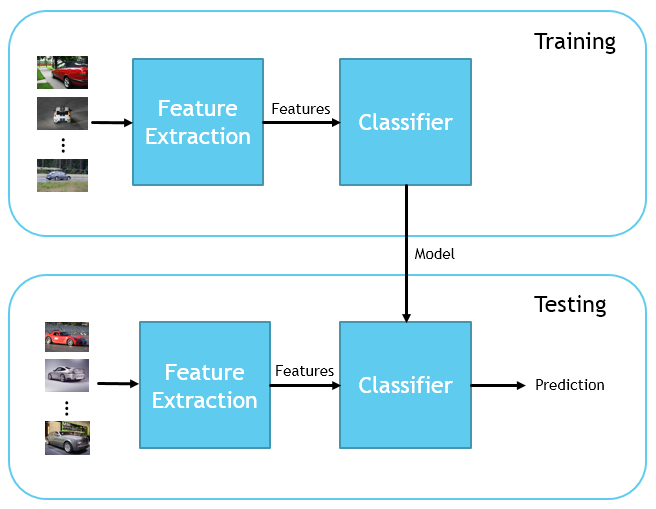
\includegraphics[scale=0.5]{image/scheme.png}
\label{fig:scheme}
\caption{Modern recognition system.}
\end{figure}

% Reason for difficulty
There are many reasons why we need some kind of feature extraction in order to perform recognition. One reason is simply because the natural representation of an image as the 2D matrix of pixel intensity values holds little to no direct information that can be used to distinguish different objects. Figure \ref{fig:car} illustrates this example. 

This is worsened by the high dimensionality of the data. A standard high definition colored image of size 1280x720 has 2,764,800 dimensions. Meanwhile the amount of training data rarely exceeds or even matches this number. This curse of dimensionality can make the training phase to become slow and hard.

\begin{figure}[h]
\centering
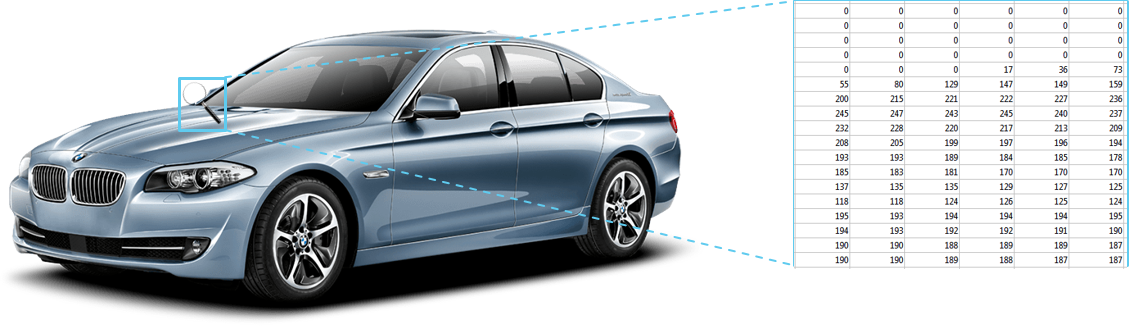
\includegraphics[scale=0.4]{image/car.png}
\label{fig:car}
\caption{The image as 2D matrix of pixels.}
\end{figure}

Furthermore, there are many variations which makes same identical objects to have very different appearances in the image. This can be due to viewing changes (translation, rotation, or scale change), change of illumination, occlusion, and clutter. There are also intrinsic difference between objects from the same class. Figure \ref{fig:cars} illustrates this example.

\begin{figure}[h]
\centering
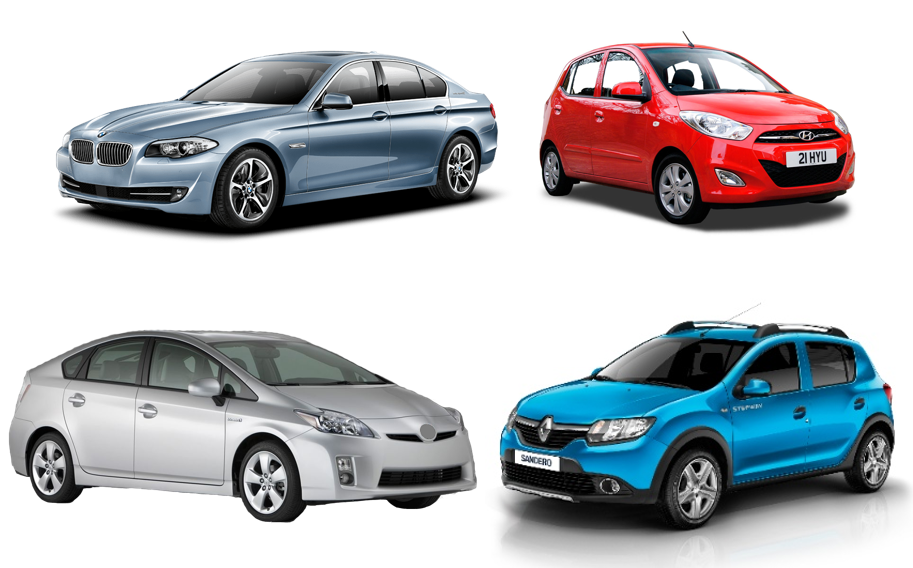
\includegraphics[scale=0.4]{image/cars.png}
\label{fig:cars}
\caption{Object with different appearances, be it color or shape, from the same class.}
\end{figure}

% The importance of features
All this boils down to finding the best representation or features of the said object. An ideal representation would be highly discriminative on different classes of object but captures the intrinsic similarity between objects from the same class. It should also be invariant to the geometric transformation (translation, rotation, and scale) of the object, usually have lower number of dimension, and also fast and easy to compute.

Unfortunately, these kind of ideal features do not exist in reality. In practice, we compromise by striking a balance of using adequate number of training data and using a stronger learning algorithm to compensate for the not-so-ideal features. Figure \ref{fig:feature} shows illustration of the ideal features and the not-so-ideal features.

\begin{figure}[h]
\centering
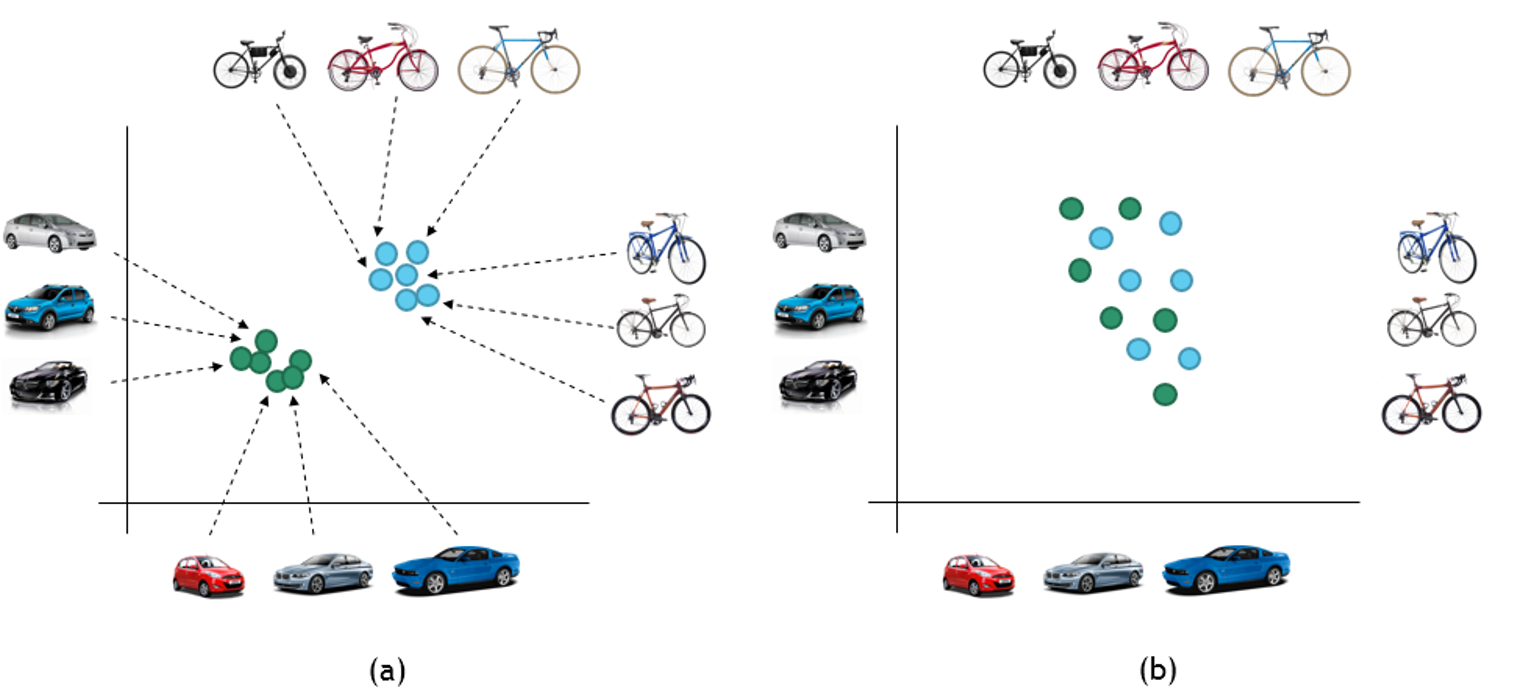
\includegraphics[scale=0.4]{image/ideal_feature.png}
\label{fig:feature}
\caption{Illustration of ideal and not-so-ideal feature representation. (a) Ideal feature should have better separability from instance from different class and closely located with object form the same class. (b) Not-so-ideal features plot is jumbled all over the place and have low separability. This, however, can be compensated by using stronger classification algorithm.}
\end{figure}

% Handcrafted features
Many studies have proposed a wide array of feature extraction techniques. Until very recently, Scale-Invariant Feature Transform (SIFT) by Lowe \cite{lowe2004sift} and Histogram of Oriented Gradients (HOG) by Dalal and Triggs \cite{dalal2005hog} are the leading technique for feature extraction and produced decent performance on benchmark dataset. Both are similar in the sense that both first compute the gradient in the image and then construct a histogram of the gradient orientation weighted by their gradient magnitude.

\begin{figure}[h]
\centering
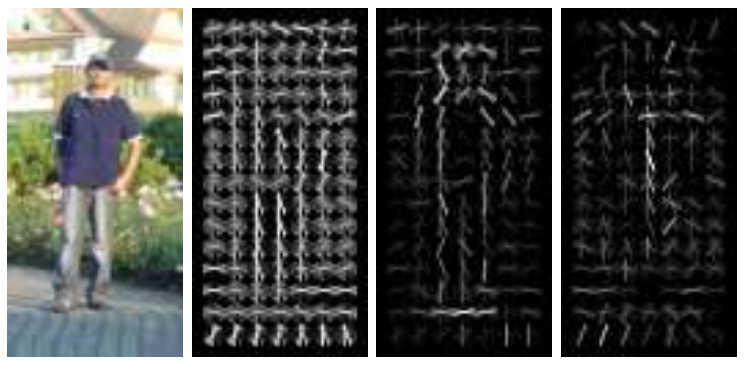
\includegraphics[scale=0.4]{image/hog.png}
\label{fig:hog}
\caption{Illustration of HOG features applied on image of a person. Image taken from \cite{dalal2005hog}}
\end{figure}

In recent years though the trend has shifted to directly learn the features from the data. This is partly motivated by the abundance of image data, mostly coming from the internet and the ubiquity of digital cameras on mobile devices which makes it easy for users to upload their images. There are two different approaches for feature learning, the unsupervised learning and supervised learning.

Unsupervised feature learning works with image without label. It tries to learn generic features of object, regardless of their class. It is more advantageous than its counterpart because even though there are plenty of data, most of them are unlabeled. The extra effort to label them can be too expensive and time-consuming.

One technique that implement this idea is Sparse Autoencoder. It is a variant of neural network, with the number of hidden neuron fewer than the dimension of the input and output. It can be said to shaped like hourglass. Figure \ref{fig:autoencoder_architecture} shows one example of autoencoder architecture. The objective of such network is to encode the image with fewer parameter and then try to decode it again and reconstruct to get the original image. It will forces the network to learn compressed, low-dimensional representation of the input. Figure \ref{fig:autoencoder} illustrates some example features learned from this network.

\begin{figure}[h]
\centering
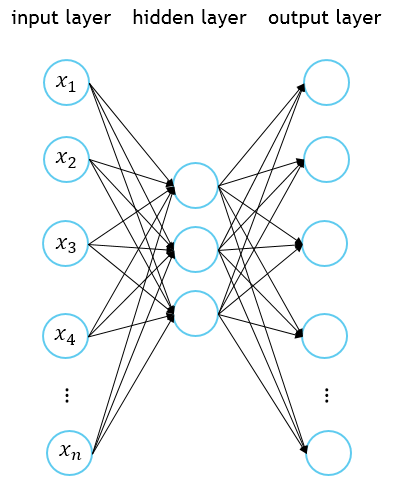
\includegraphics[scale=0.5]{image/autoencoder_architecture.png}
\label{fig:autoencoder_architecture.png}
\caption{One example of autoencoder architecture.}
\end{figure}

\begin{figure}[h]
\centering
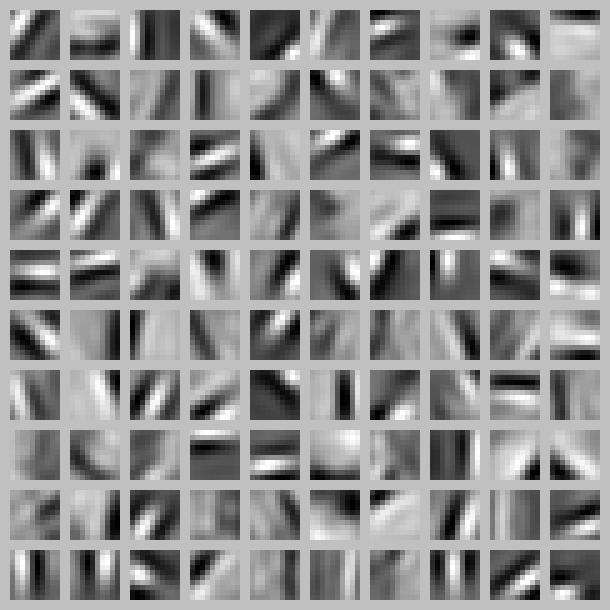
\includegraphics[scale=0.3]{image/autoencoder.png}
\label{fig:autoencoder}
\caption{The features learned from MNIST dataset. Each image correspond to edge at different location and orientation. Image taken from http://deeplearning.stanford.edu/wiki/index.php/UFLDL\_Tutorial}
\end{figure}

Supervised feature learning works with labeled images. One technique that successfully implement this idea is Convolutional Neural Network (ConvNet). This type of network architecture was originally called neocognitron, proposed by Fukushima \cite{fukushima}. Lecun et al. \cite{lecunn1999} then showed how to train such network for handwriting document classification. But this method really become popular with the success of the seminal work by Krizhevsky et al. \cite{krizhevsky2012cnn} that produced a stellar performance by beating previous state-of-the-art method by large margin, on the ImageNet large scale recognition problem \cite{imagenet}. 

Part of this success can also be attributed to the abundance of labeled training data. ImageNet contains 1.2 million labeled training images from 1000 different categories. Another factor is the advance in Graphical Processing Unit (GPU) which makes training large amount of data feasible. Combining these factors with the learning capacity of a ConvNet makes the result possible.

\begin{figure}[h]
\centering
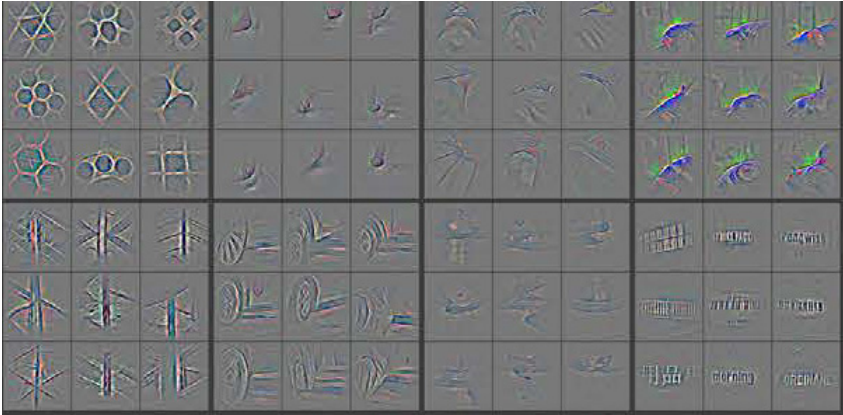
\includegraphics[scale=0.3]{image/cnn.png}
\label{fig:convnet_features}
\caption{Visualization of features learned from ConvNet. Image taken from \cite{zeiler}}
\end{figure}

Figure \ref{fig:convnet_features} shows the example of features learned from a ConvNet. Further research has shown that the features produced from the network to be highly discriminative, even across different tasks and datasets. Study by Razavian et al. \cite{razavian2014} shows that the features coming from the second last fully-connected layer of ConvNet trained on ImageNet in combination with a simple linear classifier such as Support Vector Machine (SVM) produced top and near state-of-the-art performance in many typical vision tasks such as object classification, fine-grained recognition, and image retrieval.

The result can be pushed even further by finetuning the network with the target dataset. Finetuning works by taking the previously trained network, for example, the AlexNet on ImageNet data, and retrain it with target dataset. This works particularly well, rather than training the network from beginning, especially if the target dataset has limited number of training data. This kind of learning, transfer learning, has been reported to produce better result on many occasions \cite{azizpour2014}.

\section{Proposed Study, Improvement on Object Detection}
One of the latest example that utilize the power of finetuning is the algorithm called Region with CNN (RCNN) \cite{girshick2014rcnn}. RCNN is object detection algorithm that combines the highly discriminative features from ConvNet with a better search strategy. RCNN employs the region proposal algorithm, selective search, that return ~2000 regions that is very likely to contain object. These two makes RCNN to get state-of-the-art result on benchmark dataset and made impressive improvement over previous methods.

This thesis work tries to extends the usability of RCNN. The standard RCNN needs the exact bounding box annotation for each object in the image for finetuning. However, this kind of annotation is more expensive than simply labeling the whole image. Therefore, we tries to bypass this needs and figure out a way to finetune with only whole image label. This kind of learning between the fully supervised and unsupervised is dubbed as weakly supervised learning.

The proposed general setup is as follows. First, we use a region proposal algorithm that can give confidence score that shows how likely a region to contain object. There are several possible candidates such as objectness \cite{obj} and EdgeBoxes. Hosang et al. \cite{hosang2014} provide extensive review of popular algorithm and then outline their strength and flaws. We pick top k regions and then extract them into individual image and and give the label from their source, whole image label.

These regions are then used for finetuning ConvNet that has previously been trained using ImageNet 1.2 million training images in 300,000 more iterations. This finetuned network will then be fed to the standard RCNN pipeline. The performance will be assessed using PASCAL 2007 detection dataset. It will be compared to the non-finetuned network, finetuned network with object bounding box annotation, and network finetuned with whole image.


\chapter{Literature Review}
In this chapter, we will review briefly important concepts needed on this thesis and outline their importance. First, neural network and its latest iteration, convNet, will be explained. Then, we will moved to explain the recent trend of object proposal for object detection. Then, we are going to elaborate RCNN algorithm, which combines to achieve state-of-the-art object detection on benchmark dataset. Lastly, weakly supervised object detection will be described.

\section{Convolutional Network (ConvNet)}
In this section, the development of neural network leading up to ConvNets is briefly summarized.

\subsection{Artificial Neural Network}
% Single neuron
The first neuron model is proposed by McCulloch and Pitts \cite{mcculloch1943neuron}. This model is a highly simplified version of a neuron cell in brain. It works by multiplying the input vector with the neuron's weight vector. This value is then fed into an activation function. One activation function that can be used is a step function which acts as threshold operation. If this value exceeds certain $\theta$, then this neuron fires. In other words $ a = \sum x_i w_i $ and:
\begin{equation}
y = 
	\begin{cases}
	1 & \text{if } a \geq \theta \\
	0 & \text{otherwise}
	\end{cases}
\end{equation}

This type of neuron is also called Threshold Logic Unit (TLU). Figure \ref{fig:neuron} illustrates the concept of this type of neuron.

\begin{figure}[h]
\centering
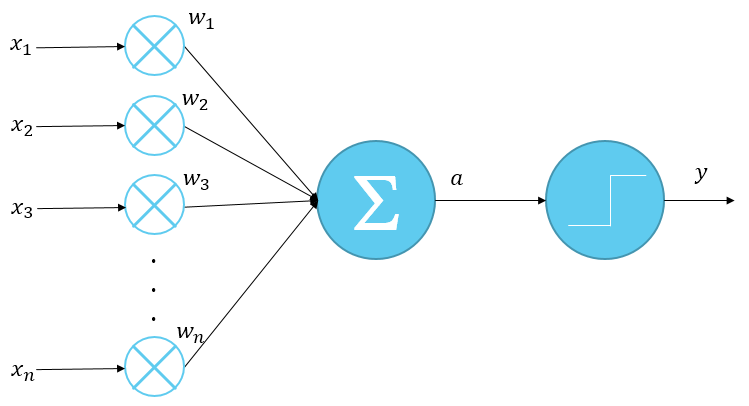
\includegraphics[scale=0.3]{image/neuron.png}
\label{fig:neuron}
\caption{Standard model of a neuron.}
\end{figure}

To update the the weight of the network to learn from the data, there are two update rules that is usually used, the perceptron rule and the delta rule. Perceptron rule was originally perceived by Rosenblatt \cite{rosenblatt1957perceptron} where to update the neuron we can just simply add the input vector to the weight vector if the output is misclassified. In other words: 
\begin{equation}
\begin{split}
\Delta w & = \alpha (t-y) \bm{x} \\
w(t+1) & = w(t) + \Delta w
\end{split}
\end{equation}
where $\bm{x}$ is the input vector, $alpha$ is the learning rate, $t$ is the target output, and $y$ is the output of the network.

There is a convergence theorem that states that if the data is linearly separable, then the perceptron learning rule will eventually converge, no matter the learning rate. However, perceptron suffer from the early stopping where if there were no training error, the network stopped learning even though the resulted network still has large validation error.

Delta rule, also known as Widrow-Hoff rule, works by minimizing a loss function. This loss function is defined as the sum of the difference between the target label and the output of the network with linear activation function. The delta rule empirically generalize better than perceptron. The update rule is defined as:
\begin{equation}
\begin{split}
\Delta w & = \alpha (t-y) g'(a) \bm{x} \\
w(t+1) & = w(t) + \Delta w
\end{split}
\end{equation}
where $a$ is the dot product between input vector and weight vector and $g'$ is the derivative of the activation function used. It is pretty similar with perceptron, with the exception of different activation function.

However, this type of networks has limitation that it can produce classifier with linear decision boundary. Even some kind of simple non-linear problem such as XOR problem cannot be solved. One way to alleviate this problem is by stacking one layer of neural network on top of other to build a multi-layer neural network. The input for the next layer is simply the output from the previous layer. The layer in the middle between input and output vector is usually called hidden layer. It has been shown that this kind of network with one hidden layer can be used to approximate any continuous function given sufficient hidden neuron \cite{cybenko1989}. Figure \ref{fig:multilayer} shows one instance of a multi-layer neural network.

\begin{figure}[h]
\centering
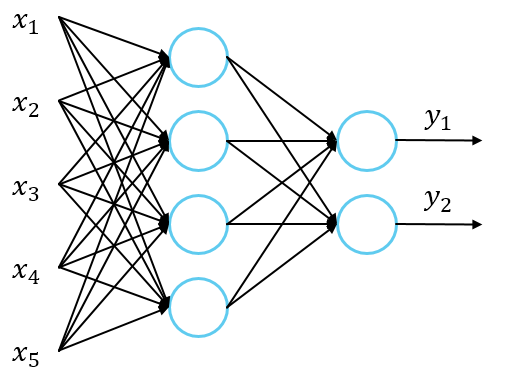
\includegraphics[scale=0.4]{image/multilayer.png}
\label{fig:multilayer}
\caption{One example of a multi-layer neural network. In this case, the input have 5 dimensions, there are 4 hidden neuron, and 2 target classes.}
\end{figure}

The caveat is then how to update the weight of the network, because we only know the error from the last layer. The found solution is by using threshold-like function, such as sigmoid function, and then performing chain rule to derive the update formula for each weight in different layers. This update formula is called Backpropogation \cite{rumelhart1986backprop}. Two popular choice for sigmoid function is $\frac{1-e^{-x}}{1+e^{-x}}$ or $arctan(x)$. Figure \ref{fig:sigmoid} shows the plot of a sigmoid function.

\begin{figure}[h]
\centering
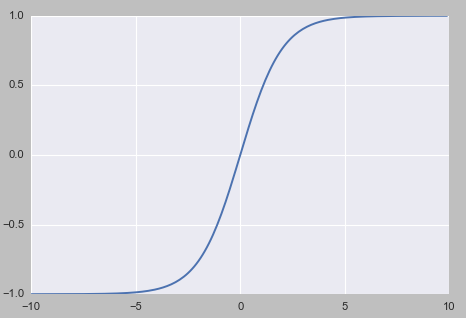
\includegraphics[scale=0.5]{image/sigmoid.png}
\label{fig:sigmoid}
\caption{Sigmoid function.}
\end{figure}

\subsection{ConvNet}
A Convolutional Neural Network (ConvNet) is a variant of the multi-layer neural network. It is inspired by the visual cortex in retina, where there are small sub-region in the cell that are highly sensitive, called receptive field. This kind of architecture is first published by Fukushima as neocognitron \cite{fukushima}. Then, paper by Lecun et al. \cite{lecunn} showed how train such network and used it to perform document handwriting recognition.

There are two different paradigms that implement this receptive field concept, which differentiates ConvNet with standard multi-layer neural network. The first concept is sparse connectivity. A neuron in this network does not need to be connected to all the neurons from the previous layer. For example, a neuron in layer $i$ is only connected to limited number of spatially adjacent neuron on layer $i-1$. Figure \ref{fig:sparse} illustrates this concept.

\begin{figure}[h]
\centering
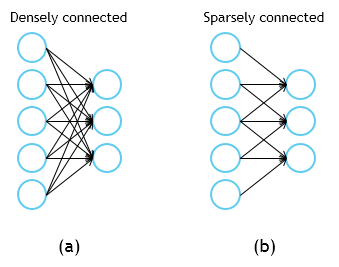
\includegraphics[scale=0.5]{image/sparse.png}
\label{fig:sparse}
\caption{Illustration between different connection. (a) Densely connected network: Connect all neurons from the previous layer to the current one. (b) Sparsely connected network: Only connect limited number of neuron. In this case it is 3 spatially adjacent neurons.}
\end{figure}

The second paradigm is shared weights. It means that the weight are the same for all neurons on the same layer, usually called a feature map. This will ensure that the distinct features will be detected regardless of their position in the input. Figure \ref{fig:shared} illustrate the concept. 

\begin{figure}
\centering
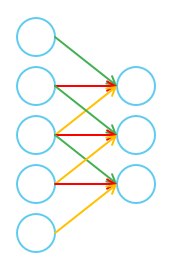
\includegraphics[scale=0.5]{image/shared.png}
\label{fig:shared}
\caption{Shared weight. Weight connection with the same color have the same value.}
\end{figure}

In one layer we can have multiple feature maps. That way, we can learn different kernels from the same input. These feature maps is stacked on top each other and thus we can learn hierarchical features, i.e. features from higher layer is constructed from features from lower layer. Figures \ref{fig:feature_map} illustrate this concept.

\begin{figure}[h]
\centering
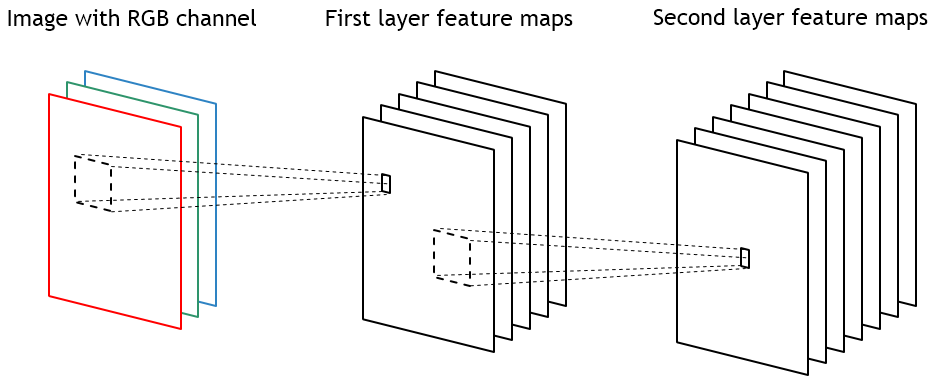
\includegraphics[scale=0.5]{image/feature_map.png}
\label{fig:feature_map}
\caption{Illustration of feature map.}
\end{figure}

This two concepts together ultimately is just a convolution operation of an image with a kernel. Therefore, in a ConvNet we are trying to learn the most discriminative, hierarchical kernel that can distinguish different objects instead of designing them by hand. It also has the advantage of having fewer parameter to train than a fully connected one.

This become the basis of the work of Krizhevsky et al. that changed the landscape of computer vision. Figure \label{fig:alexnet} shows the architecture of said network. This network is composed of 5 convolutional layers, each followed by a max-pooling layer and Rectified Linear Unit (ReLU), followed by 2 fully-connected layers and lastly softmax layer to generate prediction. This network used three additional techniques to boost the performance.

\begin{figure}
\centering
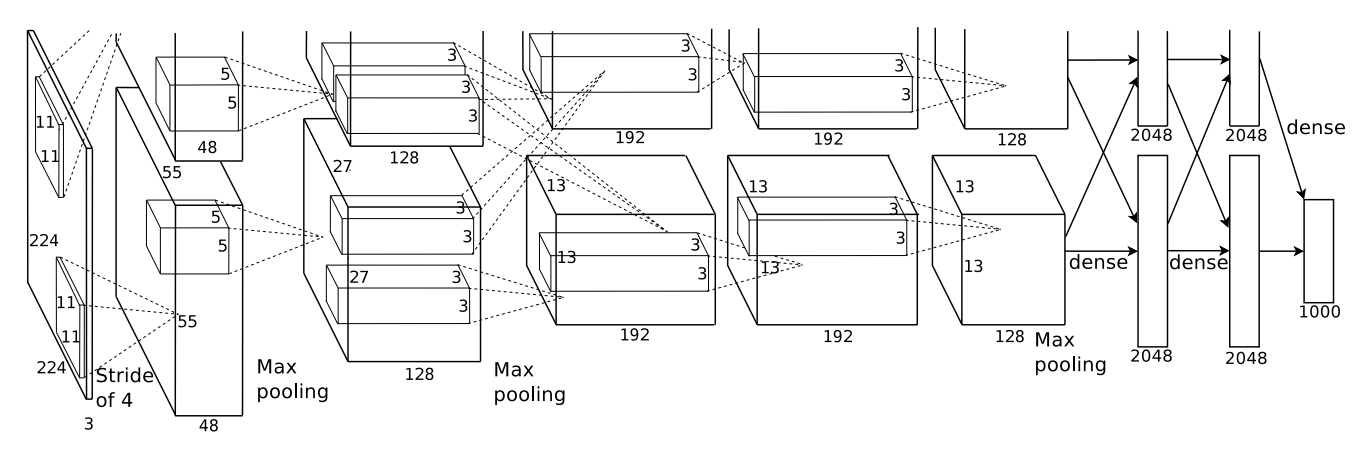
\includegraphics[scale=0.35]{image/alexnet.png}
\label{fig:alexnet}
\caption{The architecture of Alexnet.}
\end{figure}

First is max-pooling. Max-pooling partitions the image into rectangular region, and for each region, outputs the maximum value. It has the advantage of reducing the computation cost and also provide some form of translation invariance into the network.

Second, Rectified Linear Unit (ReLU) as the activation function. $max(a, 0)$. This solves the problem of vanishing gradients that often happen when training a deep, multi-layer neural network with backpropagation. As the gradient goes deeper from the output layer to the hidden layer, the gradient value quickly diminish to zero which makes the network slow to learn.

\begin{figure}[h]
\centering
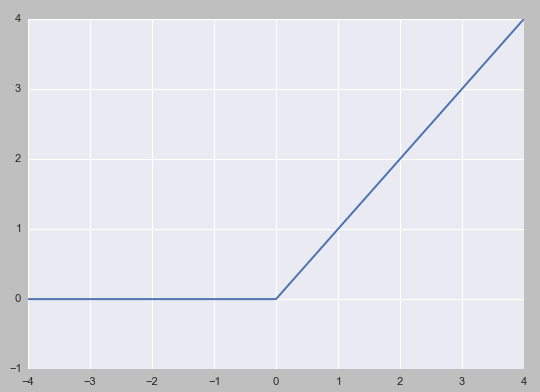
\includegraphics[scale=0.5]{image/relu.png}
\label{fig:relu}
\caption{Rectified Linear Unit. It is simply a linear activation function where value below zero is discarded and return as 0.}
\end{figure}

Third, Dropout as regularization method to prevent overfitting. This is done by setting the output of the neuron to 0 with 50\% probability. As a result it prevents neuron co-habitation and forces each neuron to independently learn the robust features.

This model is trained using GPU for 2 weeks with 1.2 million training data, trained with stochastic gradient descent with over 300,000 iterations, and achieved state-of-the-art performance on ImageNet Large Scale Visual Recognition Competition (ILSVRC) \cite{alexnet} with a large margin, over 10\% different than the previous winner.

What makes this kind of network powerful is by using deep, multi-layer neurons, hierarchical features can be learned. The lower layer can learn basic primitive such as edge and corner. This low level feature are then combined in higher layer into a more complex, higher level of representation. Figure \ref{fig:convnet_features} shows this illustrations.

\begin{figure}[h]
\centering
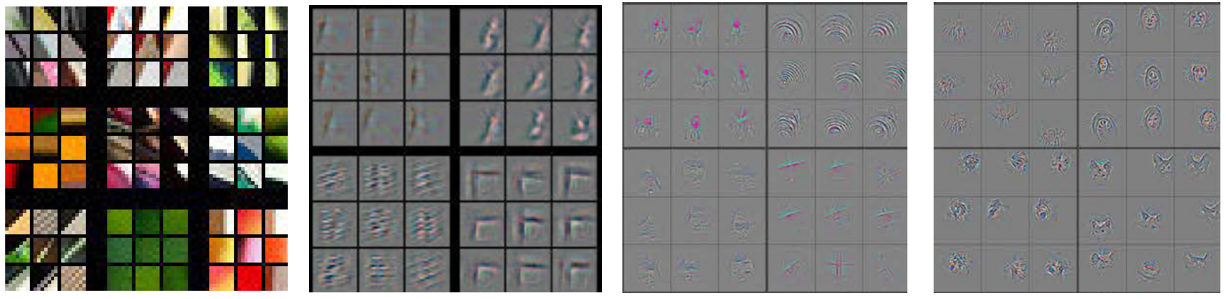
\includegraphics[scale=0.5]{image/convnet_features.png}
\label{fig:convnet_features}
\caption{Features learned from ConvNet, layer by layer. Notice that early layer (left side) learn different edge color and latest layer (right side) learn higher concept such as face of person and cat. Taken from \cite{zeiler}}
\end{figure}

\subsection{ConvNet as Black-box feature descriptor}
ConvNet works great with ImageNet dataset. However, to train network this large with hideous number of parameter, a large number of training data and computation time and power is also required. This is not a problem with ImageNet, as it contains around 1.2 million training images, sufficient to train AlexNet with 60 million parameters. Other dataset and different vision task might not have enough data.

However, rather surprisingly, it has been discovered that features produced from the last layer of a pre-trained AlexNet with ImageNet is highly discriminative. Study by Razavian et al. \cite{razavian} even shows that this features is across different vision task, such as scene and fine-grained classification. All that you need to do is to perform forward pass and then train an SVM on top of that and you can get state-of-the-art performance from it.

The performance can be pushed even further using the so-called Finetuning. Finetuning is performed by taking the previously trained network, replacing the last layer, and then training with the new target dataset. Usually the learning rate is reduced for every other weights except the last replaced layer. It has been shown that this increase the accuracy for several percent.

\section{Object Proposal}
% Traditional approach
There is a big shift in object detection world. Previously, a densely sampled sliding window is taken at all possible position and scale. It worked well, for example in the case of face detection \cite{violajones}. But when we start to take into account general object detection with different aspect ratio, the search space is simply become too big to fully explore. A standard image can produce up to million of windows to be evaluated. This can become prohibitively too slow to process. Figure \ref{fig:sliding_windows} illustrates the sliding windows concept.

\begin{figure}[h]
\centering
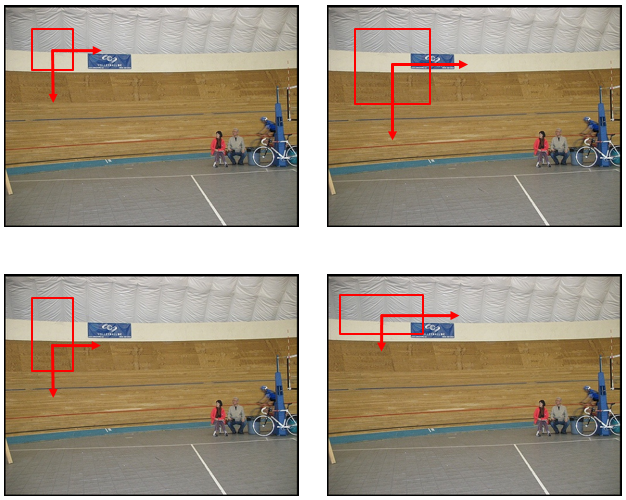
\includegraphics[scale=0.5]{image/sliding_windows.png}
\label{fig:sliding_windows}
\caption{Illustration of sliding windows approach.}
\end{figure}

% object proposal
Recent approach prefer to generate 1000-2000 candidate windows with high likelihood to contain object. The criteria to generate this boxes vary between algorithm, for example, by exploiting segmentation. It has the advantage of significantly speeding up the detection process. It can also produce better result by reducing the number of false positive rate. Figure \ref{fig:proposal} shows one example of object proposal applied to one image. Some notable object proposal algorithms will be briefly explained here.

\begin{figure}[h]
\centering
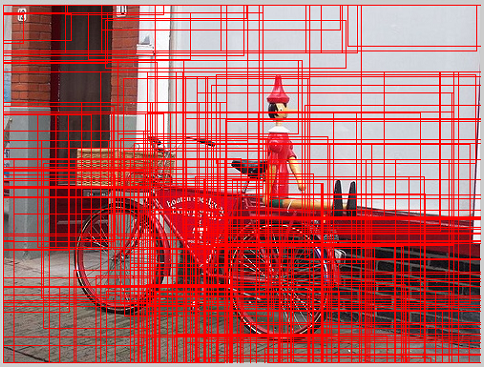
\includegraphics[scale=0.5]{image/proposal.png}
\label{fig:proposal}
\caption{Example of object proposal. Notice that the rectangle is concentrated at the lower part of the image where the object is located instead of upper part which consists of only background.}
\end{figure}

% Explain objectness
Objectness \cite{alexe2012objectness} tries to create generic object measure to distinguish object windows from background ones. It use multiple cues such as multi-scale saliency, color contrast, and edge density. It also introduces a new criterion based on the location and size of the window int he image itself, ignoring the pixels value inside the windows. It can generates up to 2000 windows in 4 seconds, in average.

% Explain selective search
Selective Search \cite{selectivesearch} performs hierarchical grouping from oversegmented region produced from Felzenszwalb and Huttenlocher graph segmentation algorithm \cite{felzenszwalb}. The grouping is done based on multiple criterion, such as color similarity, texture similarity, size (small regions should be fused with another small regions first), and fill to close gaps between regions. Higher number of proposal is obtained from combining the result from different parameters of such grouping. Figure \ref{fig:selective_search} shows the illustration of selective search.

\begin{figure}[h]
\centering
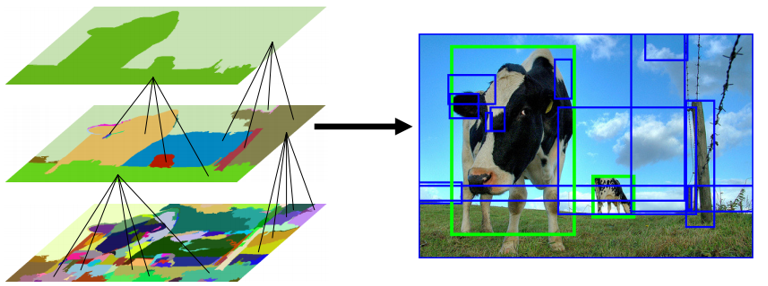
\includegraphics[scale=0.5]{image/selective_search.png}
\label{fig:selective_search}
\caption{Illustration of Selective Search steps. Image taken from \cite{uijlings2014selective}}
\end{figure}

% Explain Binarized Normed Gradient (BING)
BING \cite{bing} tries to distinguish object windows by looking at the norm of the gradient of the image window after it has been resized to small fixed size (e.g. 8x8). The approximated, binarized version of this which utilize binary operation such as ADD and BITWISE SHIFT, is very fast. It can achieved up to 300 frame per second on a single laptop CPU.

% Explain EdgeBoxes
EdgeBoxes \cite{zitnick2014edgeboxes} tries to generate object bounding box proposals directly from edges. It used the observation that the number of contours fully enclosed by a bounding box shows how likely it is to contain object. It also used smart data structure to quickly generate the bounding box. Figure \ref{fig:edgeboxes} shows the illustration of this algorithm.

\begin{figure}[h]
\centering
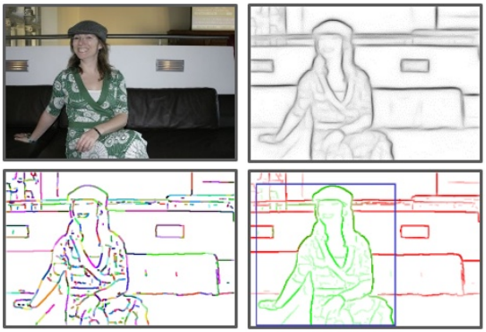
\includegraphics[scale=0.5]{image/edgeboxes.png}
\label{fig:edgeboxes}
\caption{Illutration of EdgeBoxes. First it generates edges, then perform edge grouping. Bounding boxes are then generated from this edges information. Image taken from \cite{zitnick2014edgeboxes}}
\end{figure}

% Penutup
There are a whole lot others algorithm, each with different approach and scheme. Some algorithms provided ranking as some sort of confidence whether the region contains object or not. For a complete treatment of popular object proposal algorithm, refer the work of Hosang et al. \cite{hosang}.

\section{Region with CNN (RCNN)}
Object detection is a significantly harder problem than object classification. Unlike classification, detection requires the location of the object inside the image. The second challenge is the number of labeled training data is scarce. The current amount of training data is insufficient to train a large ConvNet from scratch in order to get good feature representation.

Region with CNN features (RCNN) is the latest object detection algorithm that producing state-of-the-art result on many benchmark dataset such as PASCAL 2007 detection set and ImageNet detection problem. RCNN first solve the localization problem by using bottom up region proposal to get candidate object bounding boxes. For the second problem, RCNN use pre-trained ConvNet on large dataset (ILSRVC) followed by domain-specific fine-tuning on target dataset (PASCAL).

The general framework of RCNN is as follows. First, RCNN use class-independent region proposal algorithm such as Selective Search to generate around 2,000 proposals for each image. Then each region is warped to a fixed size to match the size of the input of the ConvNet. The features from the last fully-connected layer are then extracted. This features is then classified using pre-trained SVM classifier. Figure \ref{rcnn} shows the diagram of the RCNN system.

\begin{figure}[h]
\centering
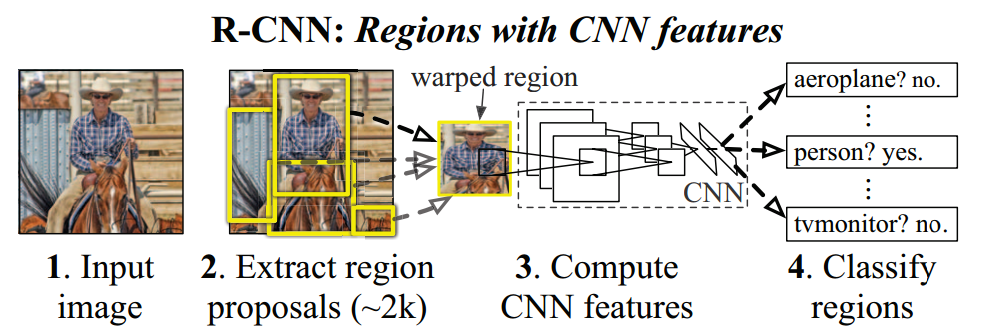
\includegraphics[scale=0.5]{image/rcnn.png}
\label{fig:rcnn}
\caption{The RCNN system.}
\end{figure}

\section{Weakly Supervised Object Detection}
Object detection algorithms usually need the object bounding boxes annotation to train the detector. However, this kind of data is rarely available and it is more expensive to obtain compare to whole image label. Therefore, it is beneficial if we can train a detector without this additional annotation. Techniques that implement this kind of data is termed weakly supervised object detection. Here we give brief overview for some state-of-the-art algorithms in this field.

Work by Wang et al. \cite{wang2014lcl}, called Latent Category Learning (LCL), try to learn hidden subcategory for each region using probabilistic Latent Semantic Analysis. He then picked the most discriminative subcategories. The next step is following the same pipeline as RCNN, where it used ConvNet as representation and SVM for classification.
Cinbis et al. \cite{cinbis2014mil} treat this problem as multiple instance learning and use multi-fold approach where the data is divided into train and validation part. The SVM is trained on training data and then it is used to refine the localization of the validation part. This process is performed iteratively for every fold.

To implement a true weakly supervised, both the finetuning and classifier should not need the bounding box annotation. However, due to time constraint, in this work we only try to finetune the network in weakly supervised way. SVM training in weakly supervised fashion is left as future work.

\chapter{Experiment and Result}
This section will briefly. First the dataset used in the experiment will be briefly introduced. Then all the code necessary will also be explained. The experiment setup and designs and their result will be elaborated. It will then be closed with a discussion regarding the results and what to make out of it.

\section{Dataset}
The dataset used in the experiment is PASCAL Visual Object Classes Challenge 2007 (VOC2007) for detection task \cite{pascal2007}. This dataset contains 9963 images, divided into 2501 images for training, 2510 for validation, and 4952 for testing. There are total 24,640 annotated objects from 20 different visual classes. The classes can be divided roughly into several subcategories:
\begin{enumerate}
\item Person: person.
\item Animal: bird, cat, cow, dog, horse, sheep.
\item Vehicle: aeroplane, bicycle, boat, bus, car, motorbike, train.
\item Indoor: bottle, chair, dining table, potted plant, sofa, tv/monitor.
\end{enumerate}

The measurement used is average precision (AP). It is computed from taking the average of precision value at 11 different recall level. This is a better measure than a simple accuracy due to the imbalance of the data. Figure \ref{fig:pascal} shows some example image from this dataset.

\begin{figure}
\centering
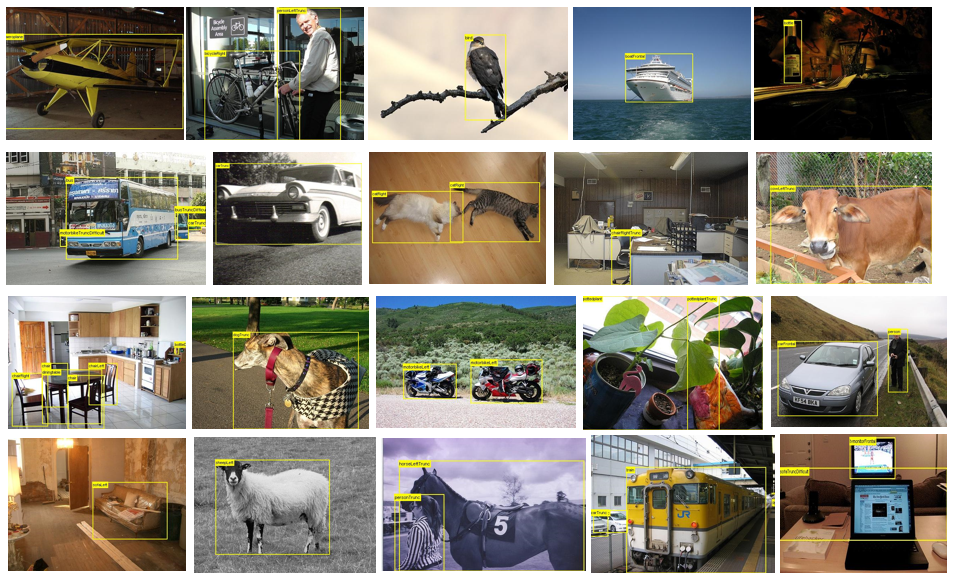
\includegraphics[scale=0.5]{image/pascal_samples.png}
\label{fig:pascal}
\caption{Some samples image from VOC2007 all 20 classes.}
\end{figure}

\section{Software}
For the implementation of the ConvNet, we are using Caffe deep learning framework \cite{caffe}, originally developed by Jia and now maintained by Berkeley Vision and Learning Center. Caffe holds several advantages compared to alternative library such as MatConvNet and theano. It is designed to be able to perform experiment with different architecture and parameter with only changing the prototext file, without touching any code at all. It is also pretty easy to switch between CPU and GPU, depending on available hardware. It also boasts fast speed (up to 1 ms for one forward pass) and has live community and extensive documentation.

Caffe also provides several pre-trained ConvNet models and architectures. We specifically use the model called BVLC Reference that follows the architecture of alexnet with minor variation. This network will then be referred throughout the rest of this thesis as caffenet. There is also a model zoo, where researchers and scientist worldwide can participate uploading new and different model that can be used with Caffe software. However, testing different architecture for the detection task is out of the scope of this thesis.

As for the RCNN code itself, the author provide it online in a github repository: http://github.com/rbgirshick/rcnn. We just need to provide a model file as one argument to the function. For the classification part, we use LibLinear SVM \cite{liblinear}, available at: http://www.csie.ntu.edu.tw/~cjlin/liblinear/. For region proposal, we use Selective Search, EdgeBoxes, and Bing. All of them are available online.

\section{Experiment}
We will perform several experiments. The first set of experiment will try to reproduce the result of RCNN on VOC07 dataset. For the second set of experiment, we will look at the effect of several strategies of finetuning the network with weak label.

\subsection{Baseline}
\subsubsection{First experiment, Lower bound}
The first experiment will be using RCNN code with pre-trained caffenet. The average precision for all 20 classes are listed on Table \ref{tab:lower}. The precision-recall curve for all classes is shown on Figure \ref{fig:pr_lower}.

\begin{table}[h]
\begin{tabular}{lllllllllllllllllllll}
aero  & bike  & bird  & boat  & bottle & bus   & car   & cat   & chair & cow   & table & dog   & horse & mbike & person & plant & sheep & sofa  & train & tv    & mAP    \\
\hline
57.62 & 60.48 & 42.21 & 31.31 & 25.41  & 52.64 & 59.58 & 49.42 & 22.1  & 41.67 & 34.97 & 45.43 & 45.72 & 55.32 & 42.06  & 22.47 & 46.65 & 34.49 & 51.44 & 58.87 & 43.993
\end{tabular}
\end{table}

\begin{figure}[h]
\centering
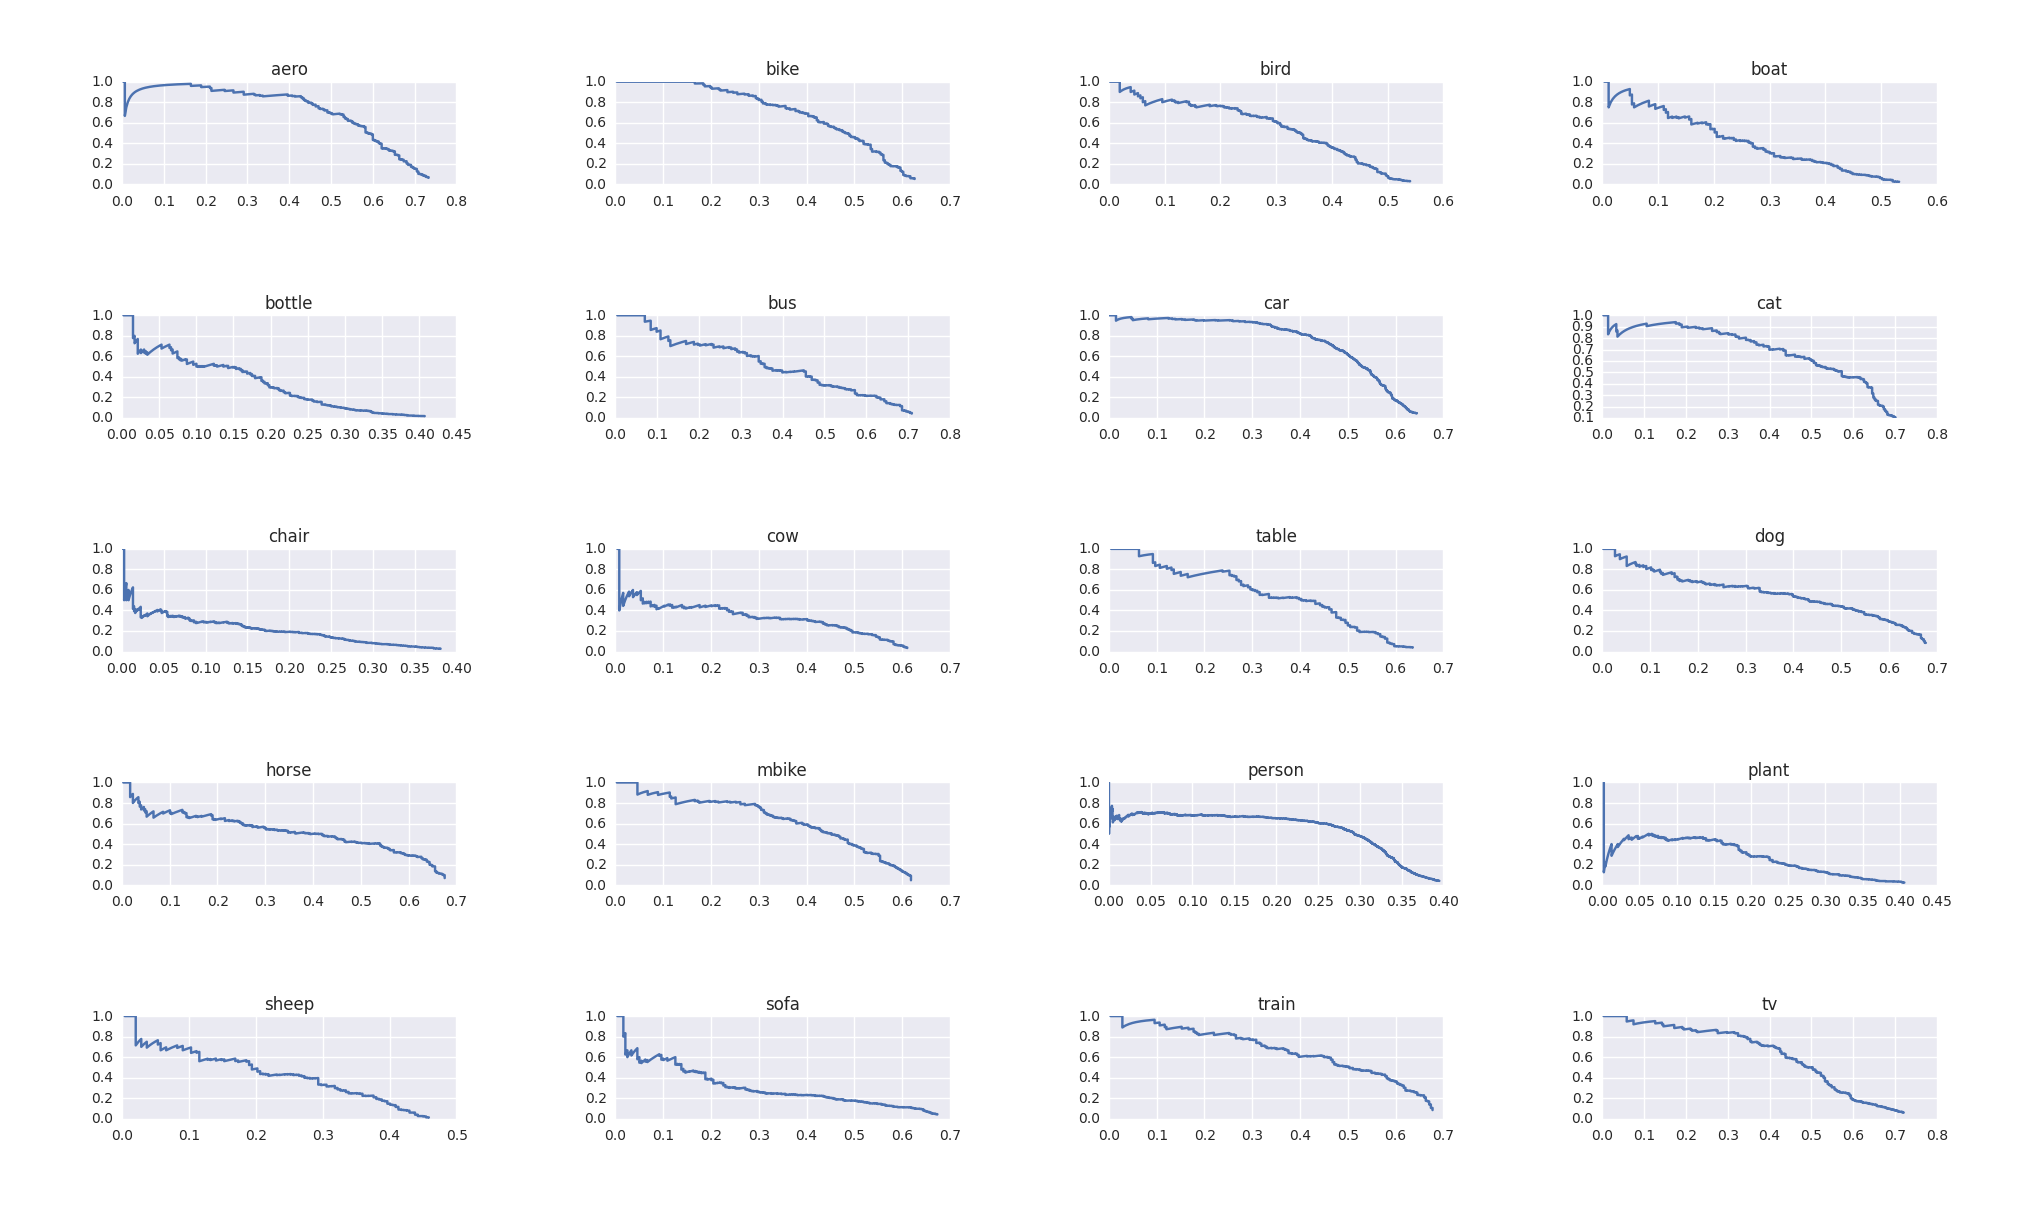
\includegraphics[scale=0.3]{image/pr_lower.png}
\label{fig:pr_lower}
\caption{The precision-recall curve for all 20 classes.}
\end{figure}

This result will act as lower bound for the rest of the experiment. It is hoped that any finetuning performed on the 

\subsubsection{Second Experiment, Upper bound}
For the second experiment, the caffenet model will first be finetuned using VOC2007 dataset.

From each image, around 2000 windows are extracted using Selective Search region proposal algorithm. The regions are chosen as positive training data for finetuning if they at least have 0.3 overlap with any object bounding boxes. Any region with 0 overlap is picked as negative data. The finetuning is 100,000 iterations, with 0.001 learning rate $\alpha$ for all layers except the last one, which is 0.01. The learning rate is reduced every 20,000 iterations by multiplying the current $\alpha$ with gamma value of 0.1. Figure \ref{fig:finetune_rcnn} shows the plot of loss and accuracy at each iteration.

\begin{figure}
\centering
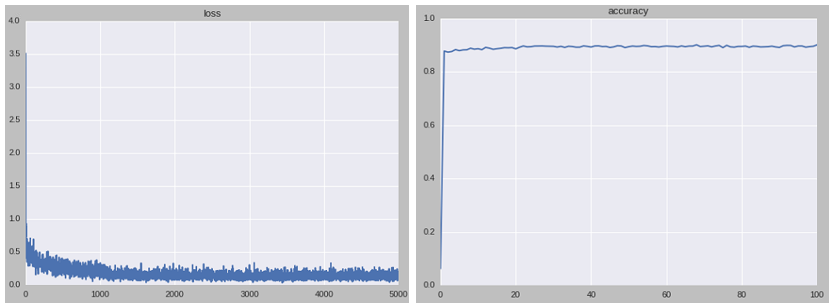
\includegraphics[scale=0.5]{image/finetune_rcnn.png}
\label{fig:finetune_rcnn}
\caption{Loss and Accuracy plot at finetuning.}
\end{figure}

This finetuned network is then used for the RCNN code input. The average precision for all classes is listed in table \ref{tab:finetune_rcnn}.

\begin{table}[h]
\label{tab:finetune_rcnn}
\begin{tabular}{lllllllllllllllllllll}
aero  & bike  & bird  & boat  & bottle & bus   & car   & cat   & chair & cow   & table & dog   & horse & mbike & person & plant & sheep & sofa  & train & tv    & mAP     \\
57.62 & 60.48 & 42.21 & 31.31 & 25.41  & 52.64 & 59.58 & 49.42 & 22.1  & 41.67 & 34.97 & 45.43 & 45.72 & 55.32 & 42.06  & 22.47 & 46.65 & 34.49 & 51.44 & 58.87 & 43.993  \\
65.83 & 68.62 & 49.64 & 36.53 & 29.31  & 65.09 & 70.58 & 58.04 & 32.63 & 61.89 & 48.67 & 57.25 & 59.53 & 64.88 & 53.34  & 34.63 & 56.34 & 48.4  & 57.28 & 64.73 & 54.1605
\end{tabular}
\end{table}

There is a solid improvement of 8\% from previous experiment. This add to the mounting evidence that finetuning with target dataset helps, however little.

\subsection{Weakly Finetuning}
In this section we now try to finetune the caffenet with only whole image label, without the bounding box annotation. There are several strategies that can be chosen and they are will be explained in the next section.

\subsubsection{First model, whole image}
For the first model, we just simply finetune the caffenet with whole image. Because one image can have multiple objects from different classes, in this experiment, we only picked image with. This reduce the number of training data to just around 3,000. We then finetuned with the same parameter as previous experiment. Figure \ref{fig:finetune_whole} shows the plot of loss and accuracy.

\begin{figure}
\centering
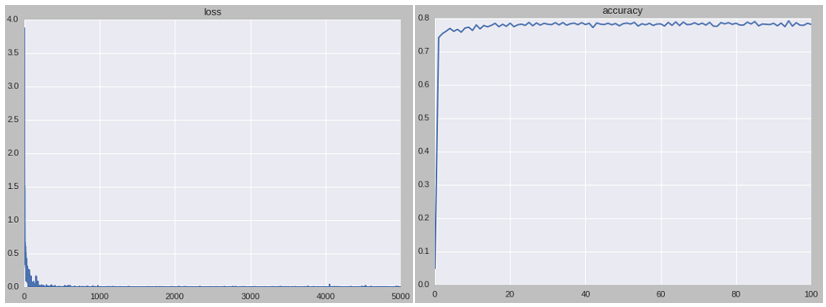
\includegraphics[scale=0.5]{image/finetune_whole}
\label{fig:finetune_whole}
\caption{Plot of Loss and Accuracy with whole image finetuning.}
\end{figure}

\begin{table}[h]
\label{tab:finetune_whole}
\begin{tabular}{lllllllllllllllllllll}
aero  & bike  & bird  & boat  & bottle & bus   & car   & cat   & chair & cow   & table & dog   & horse & mbike & person & plant & sheep & sofa  & train & tv    & mAP     \\
57.62 & 60.48 & 42.21 & 31.31 & 25.41  & 52.64 & 59.58 & 49.42 & 22.1  & 41.67 & 34.97 & 45.43 & 45.72 & 55.32 & 42.06  & 22.47 & 46.65 & 34.49 & 51.44 & 58.87 & 43.993  \\
52.91 & 60.65 & 36.06 & 32.45 & 20.97  & 46.61 & 56.24 & 42.09 & 18.92 & 38.71 & 34.1  & 41.45 & 45.23 & 55.79 & 38.92  & 25.26 & 43.91 & 28.07 & 50.01 & 51.12 & 40.9735
\end{tabular}
\end{table}

the mAP is shown on Table \ref{tab:finetune_whole}. As can be seen, even though there are small increase in several classes, overall the mAP is decreased by 4\% compared to the lower bound result.

\subsubsection{Second model}
For the second model, we tried to insert multiple. For images with multiple labels, we simply list them several times in the training file list, each time with different labels. This double the number of training data to 7,000. The finetuning process is using the same parameter as above experiment.

[plot loss and accuracy]
[table]

\subsubsection{Third model}
For this third model using region to finetune the network. We used the top 5 region for each image produced using EdgeBoxes region proposal algorithm. The region is filtered, only region with the size of at least 30\% of image size get picked as training data. The number of training data for finetuning is around 3,000. This data is then used for finetuning with the same parameter as previous experiment.

[plot loss and accuracy]
[table]

\subsubsection{Fourth model}
For the fourth model, we tried to increase the number of training data by using top 10 regions. This doubles the number into 7,000.

[plot loss and accuracy]
[table]

\subsubsection{Fifth model}
For the fifth model, we include all images with multiple labels, therefore each region can have multiple labels, just like second model. We are also using top 5 region from EdgeBoxes region proposal algorithm. The total number of training data reach more than 11,000.

[plot loss and accuracy]

The average precision can be seen on table \ref{tab:model5}.

[table]

\section{Discussion}
Based from the result of all experiment above, there are several early conclusion to be drawn. First, feature from to different task than it was trained for (detection as opposed to classification) and different dataset (VOC2007 as opposed to Imagenet). Second, finetuning with data from new, target dataset can improve the result. However, there are still difficulties to finetune for detection task if we only have label for the whole image and not the bounding box annotation.

\bibliographystyle{plain}
\bibliography{ref.bib}

\appendix
\addappheadtotoc
\chapter{Finetune}\label{appA}

This is appendix.

\end{document}
